\subsection{Truthseeker}

\subsubsection{Accuracy}
Figure~\ref{fig:accuracy} shows the accuracy of different compressors, metics, and sample selection methods.

\begin{figure*}
	% \begin{subfigure}
	% 	\centering
	% 	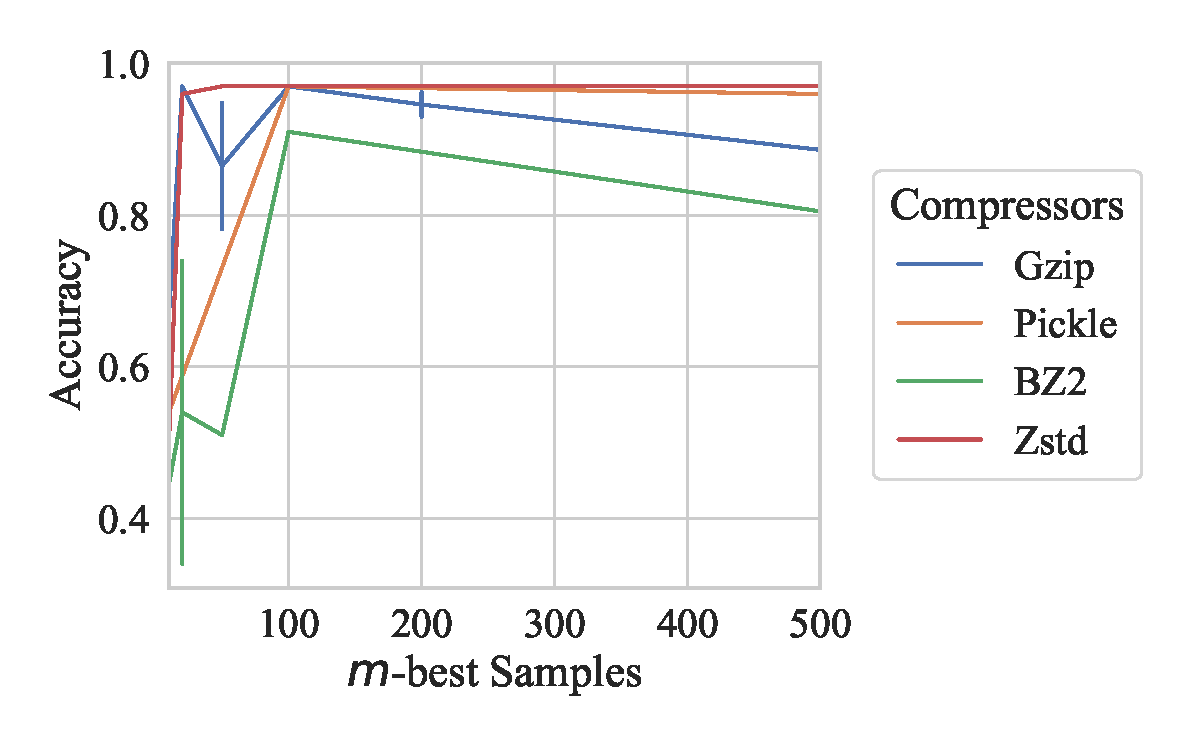
\includegraphics[width=.46\textwidth]{figs/truthseeker/compressor_vs_accuracy.pdf}
	% \end{subfigure}%
	% ~
	\begin{subfigure}
		\centering
		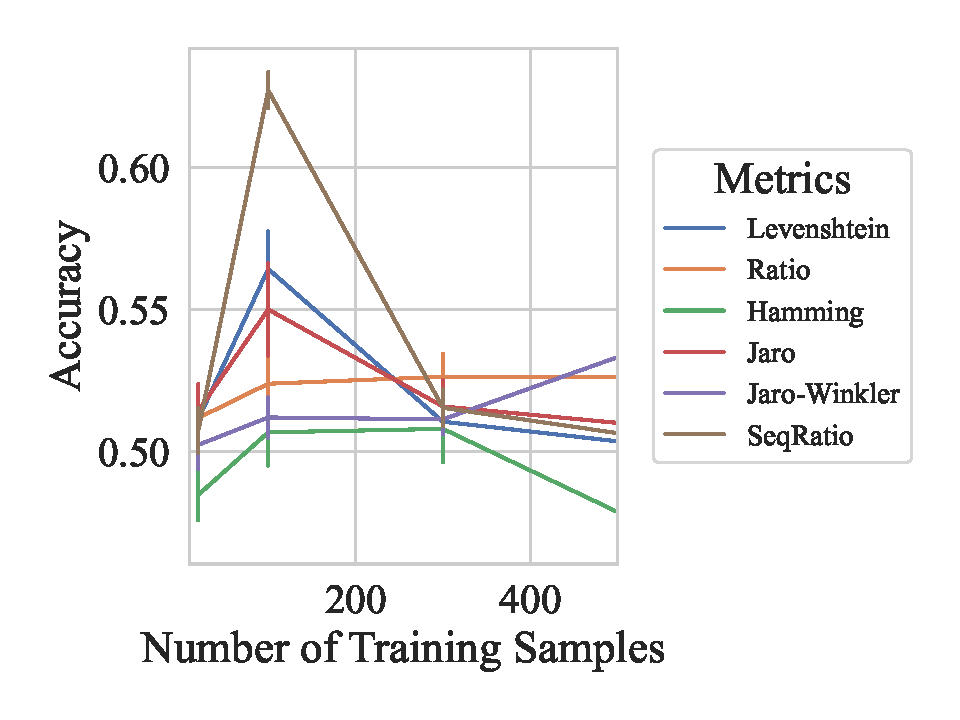
\includegraphics[width=.46\textwidth]{figs/truthseeker/string_metric_vs_accuracy.pdf}
	\end{subfigure}
	~
	\begin{subfigure}
		\centering
		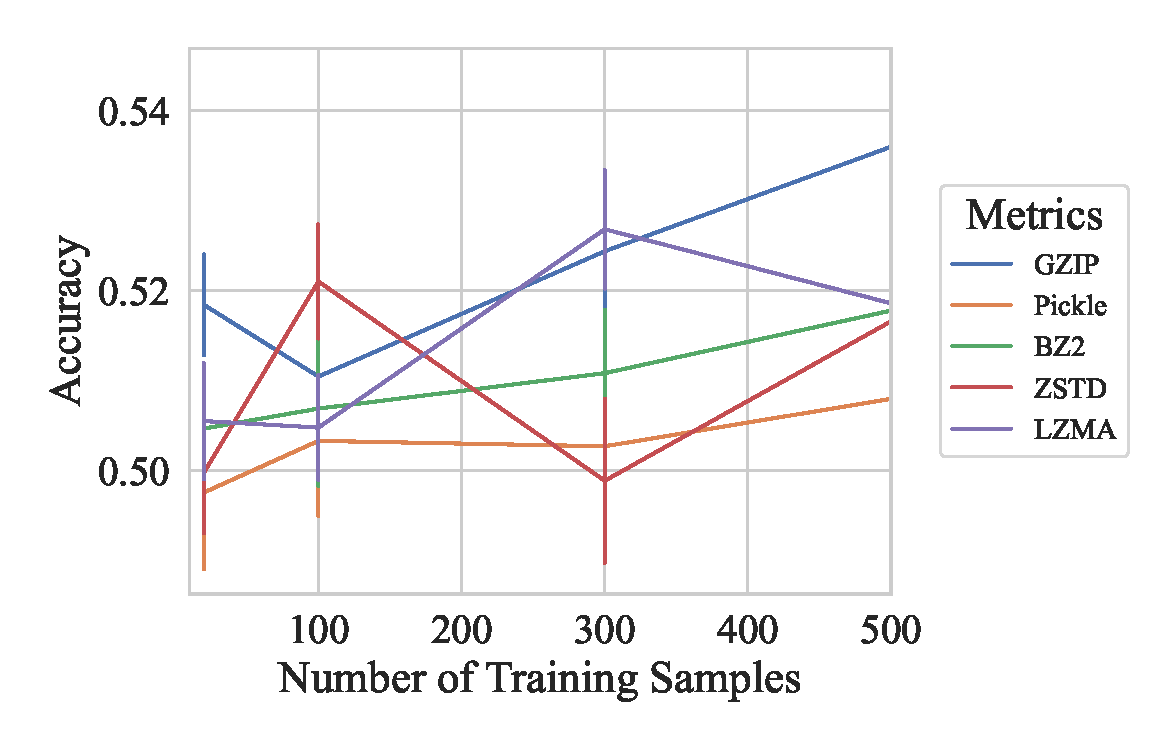
\includegraphics[width=.46\textwidth]{figs/truthseeker/compressor_metric_vs_accuracy.pdf}
	\end{subfigure}
	\caption{Accuracy across different different string kernel metrics (left), and compression methods (right).}
	\label{fig:accuracy}
\end{figure*}

\subsubsection{Training Time}

Figure~\ref{fig:training_time} depicts the training time across all the tested compressors, distance metrics, and sample selection methods.

\begin{figure*}
	% \begin{subfigure}
	% 	\centering
	% 	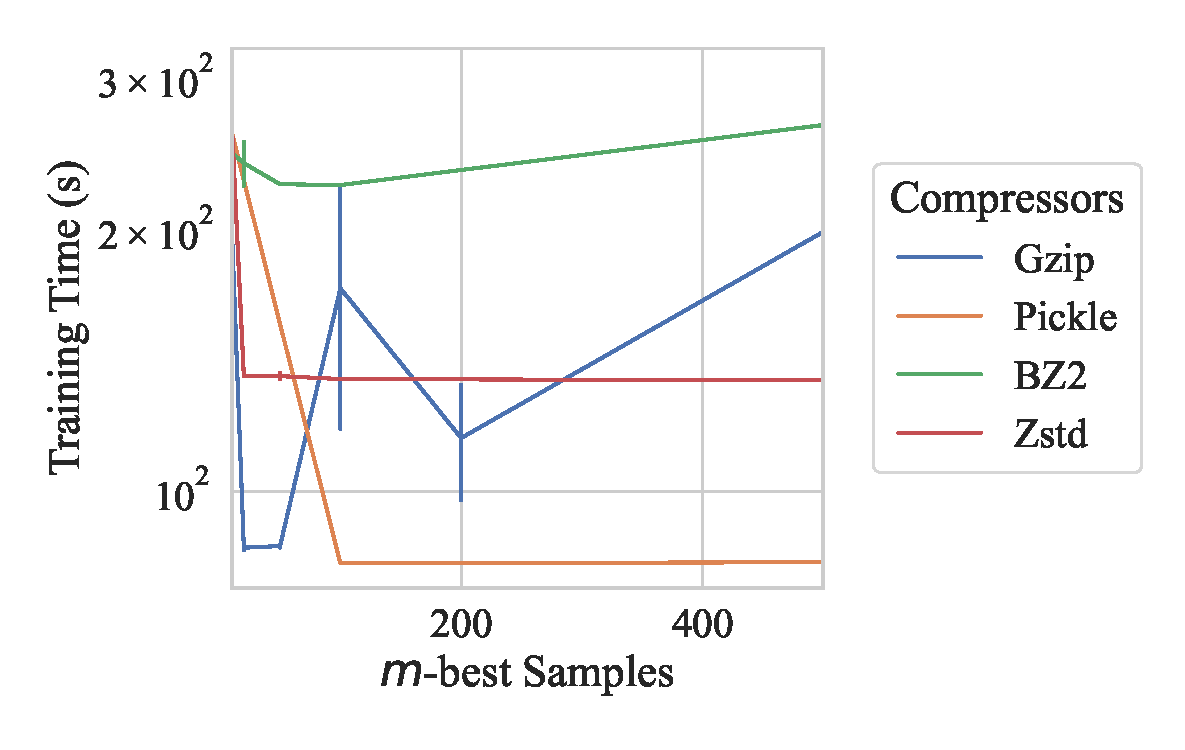
\includegraphics[width=.46\textwidth]{figs/truthseeker/compressor_vs_train_time.pdf}
	% \end{subfigure}%
	% ~
	\begin{subfigure}
		\centering
		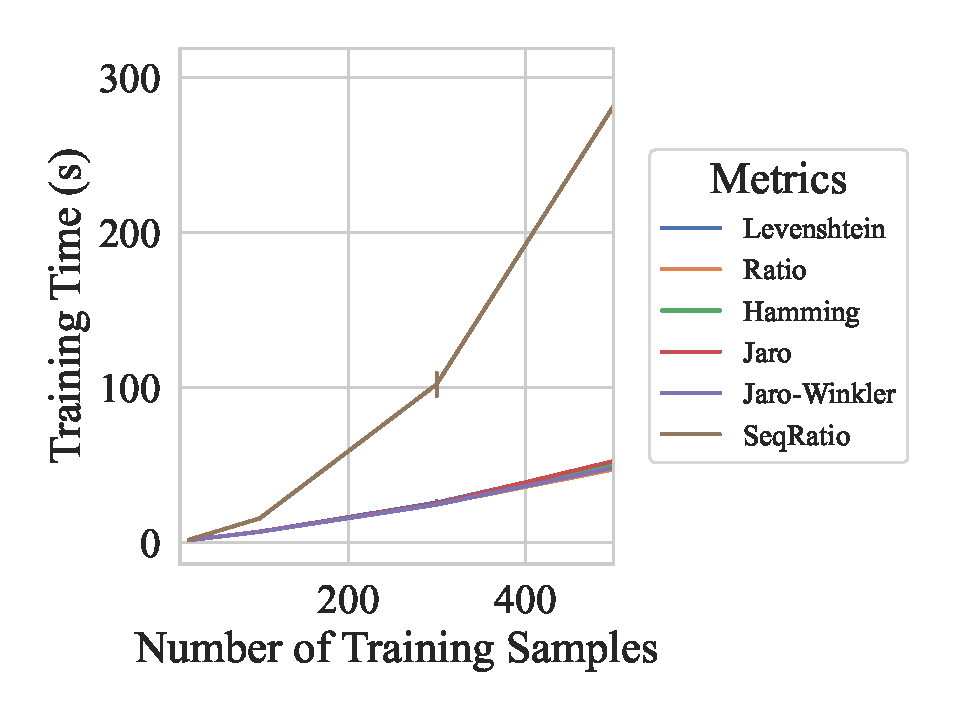
\includegraphics[width=.46\textwidth]{figs/truthseeker/string_metric_vs_train_time.pdf}
	\end{subfigure}
	~
	\begin{subfigure}
		\centering
		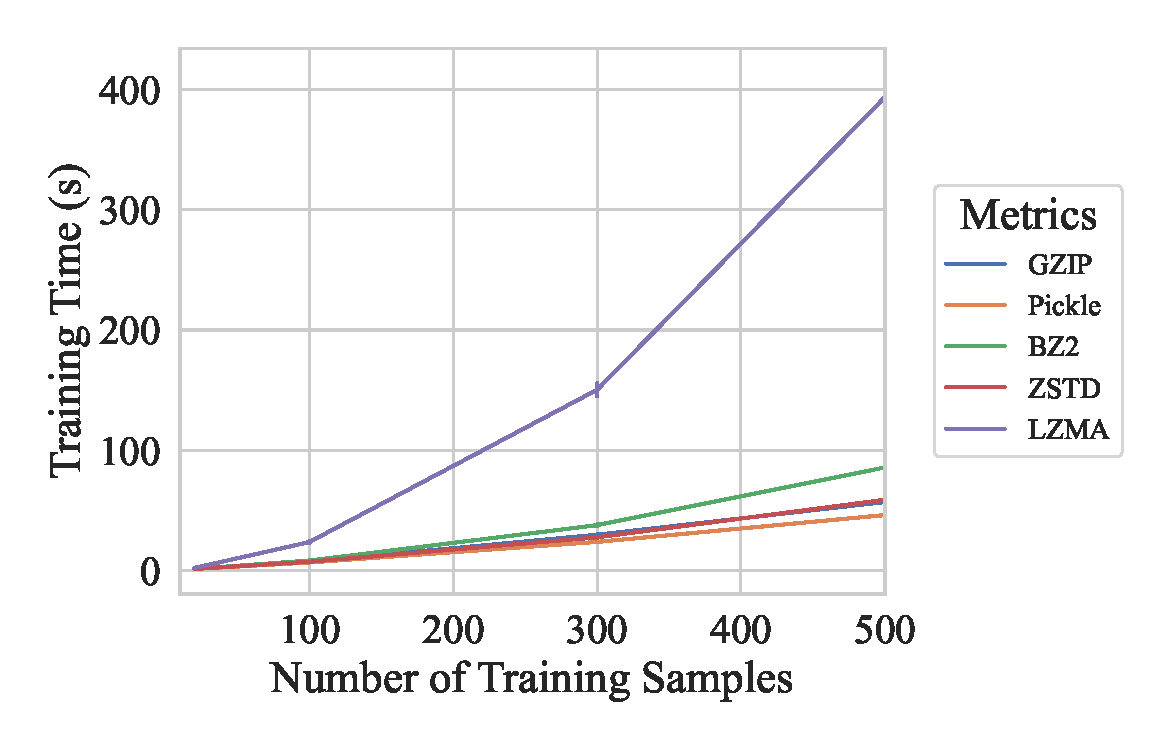
\includegraphics[width=.46\textwidth]{figs/truthseeker/compressor_metric_vs_train_time.pdf}
	\end{subfigure}
	\caption{Training time across different different string  metrics (left), and compression methods (right).}
	\label{fig:training_time}
\end{figure*}

\subsubsection{Prediction Time}

Figure~\ref{fig:prediction_time} shows the prediction time of different compressors, metics, and sample selection methods.
\begin{figure*}
	% \begin{subfigure}
	% 	\centering
	% 	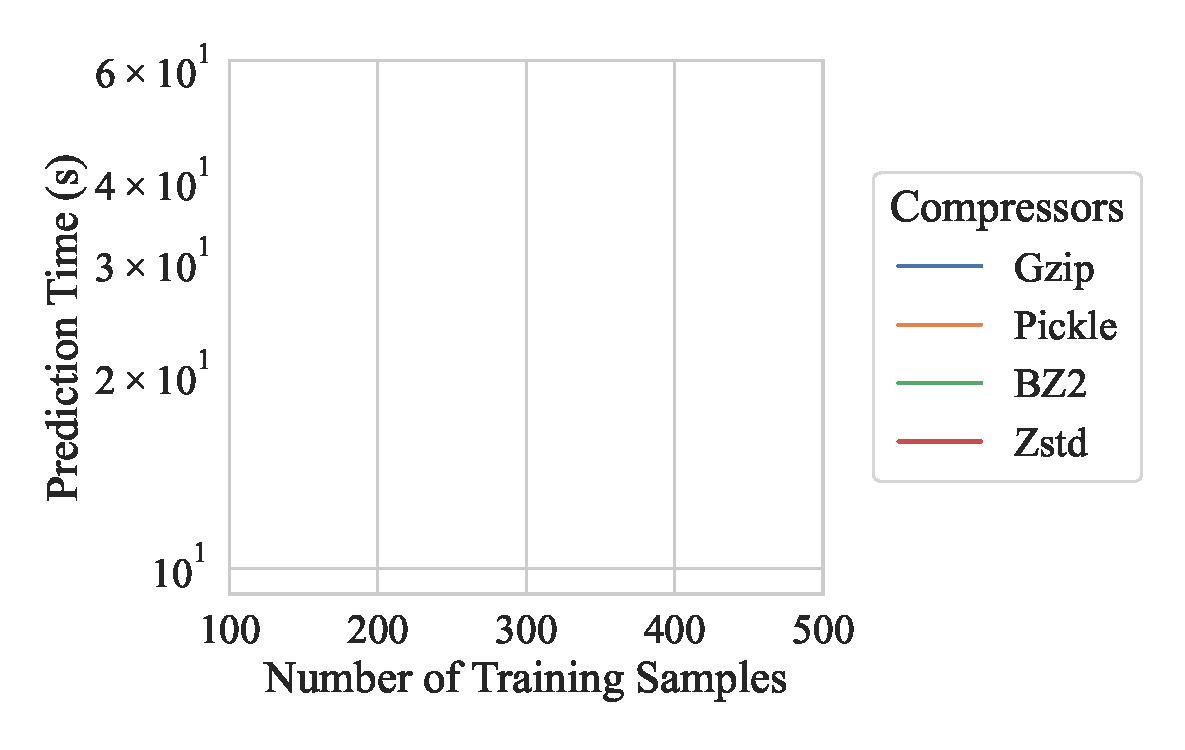
\includegraphics[width=.46\textwidth]{figs/truthseeker/compressor_vs_predict_time.pdf}
	% \end{subfigure}%
	% ~
	\begin{subfigure}
		\centering
		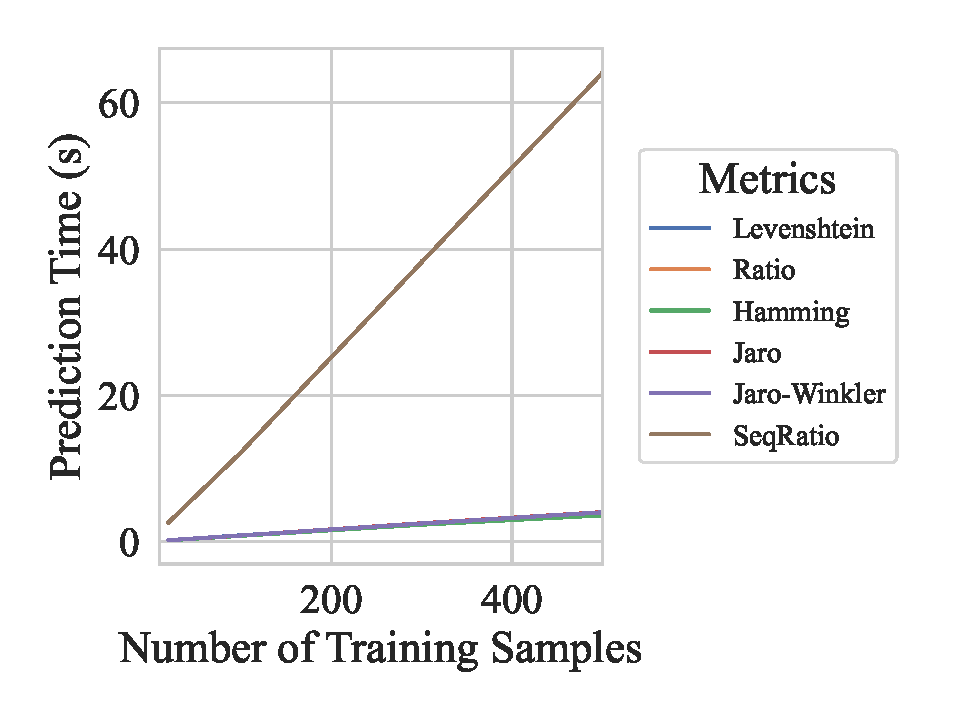
\includegraphics[width=.46\textwidth]{figs/truthseeker/string_metric_vs_predict_time.pdf}
	\end{subfigure}
	~
	\begin{subfigure}
		\centering
		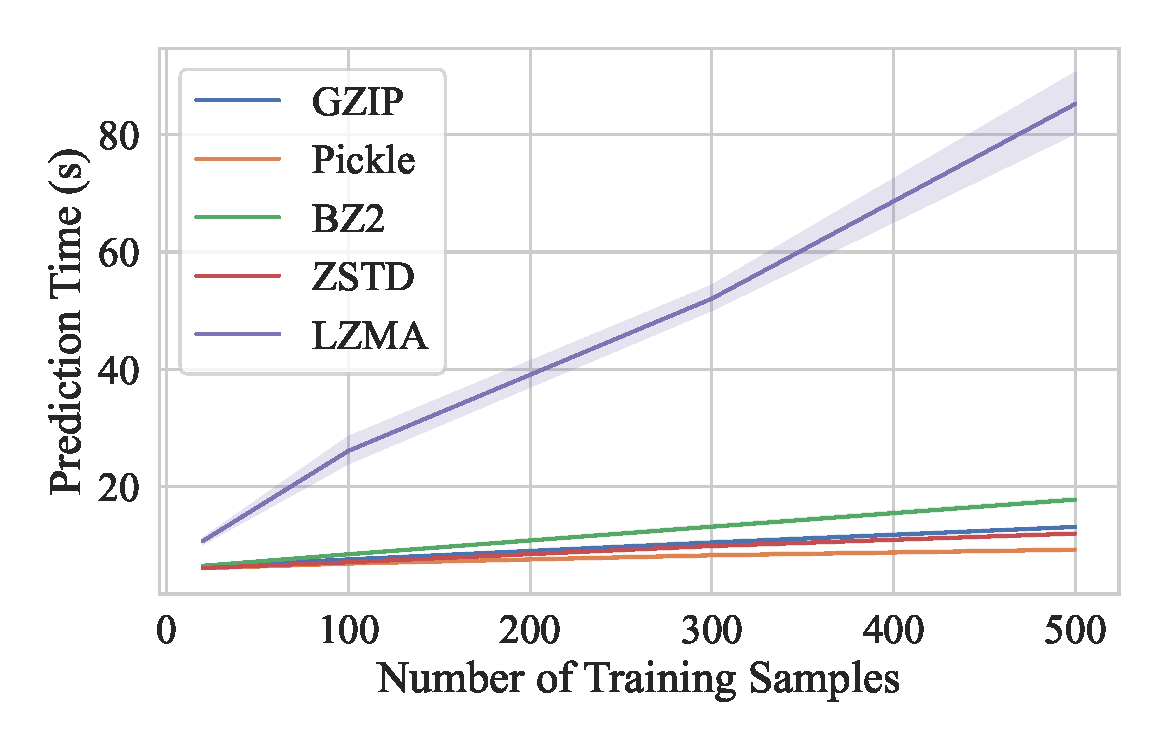
\includegraphics[width=.46\textwidth]{figs/truthseeker/compressor_metric_vs_predict_time.pdf}
	\end{subfigure}
	\caption{Prediction time across different different string metrics (left), and compression methods (right).}.
	\label{fig:prediction_time}
 
\end{figure*}

\subsubsection{Symmetry}

Figure~\ref{fig:symmetry} shows the 

\begin{figure*}
    % \begin{subfigure}
    %     \centering
    %     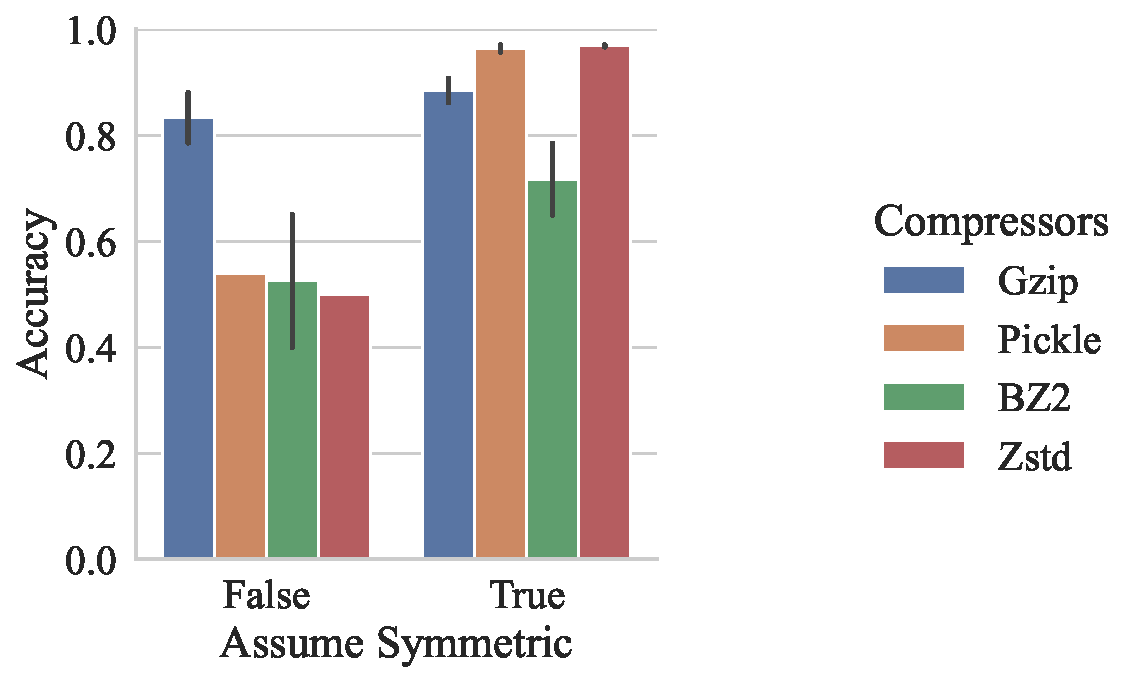
\includegraphics[width=.36\textwidth]{figs/truthseeker/symmetric_vs_compressor.pdf}
    % \end{subfigure}
    \begin{subfigure}
        \centering
        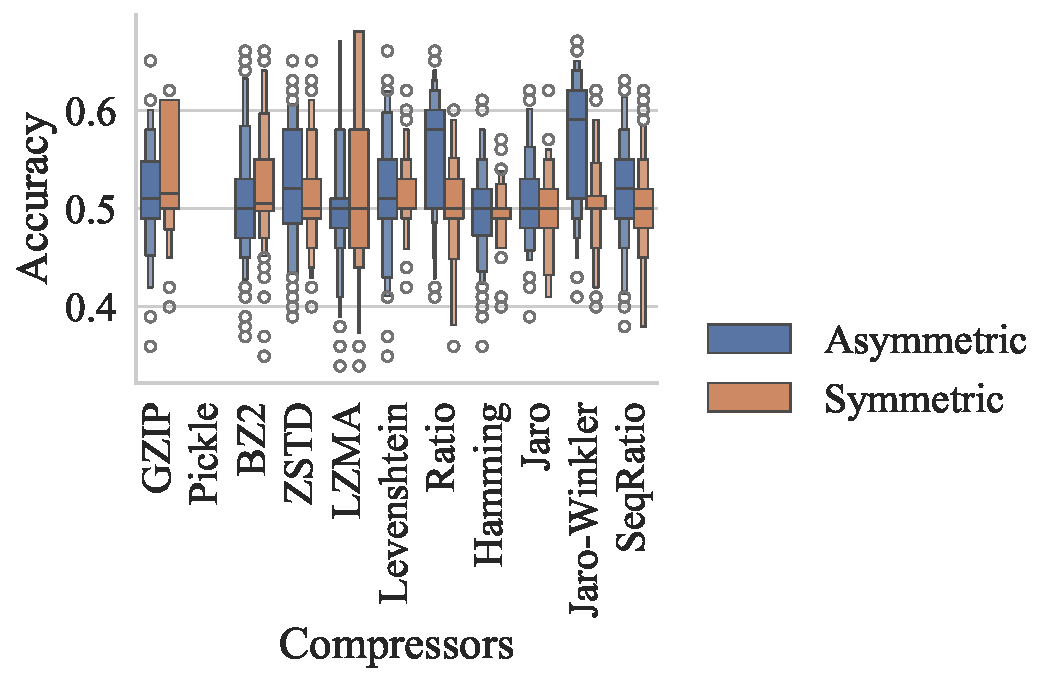
\includegraphics[width=.36\textwidth]{figs/truthseeker/symmetric_vs_metric.pdf}
    \end{subfigure}
    \begin{subfigure}
        \centering
        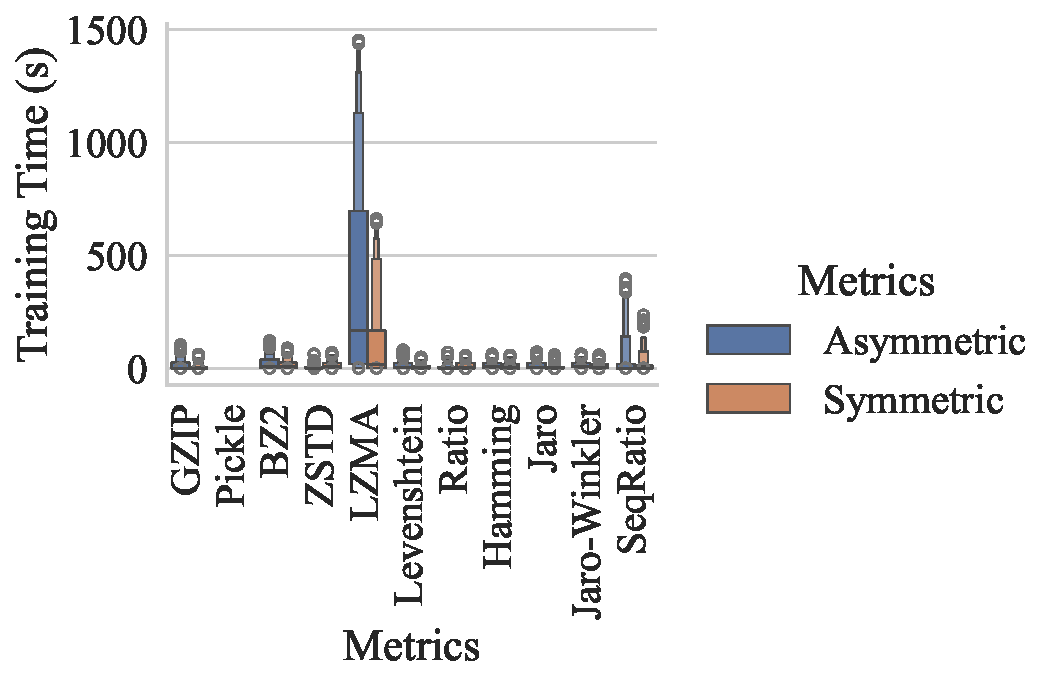
\includegraphics[width=.36\textwidth]{figs/truthseeker/symmetric_vs_metric_train_time.pdf}
    \end{subfigure}
    \caption{Accuracy across (left) and prediction time (right) across several compression methods and distance metrics with and without assuming symmetric distances.}
    \label{fig:symmetry}
\end{figure*}


\subsection{KDD-NSL}

\subsubsection{Accuracy}
Figure~\ref{fig:accuracy} shows the accuracy of different compressors, metics, and sample selection methods.

\begin{figure*}
	% \begin{subfigure}
	% 	\centering
	% 	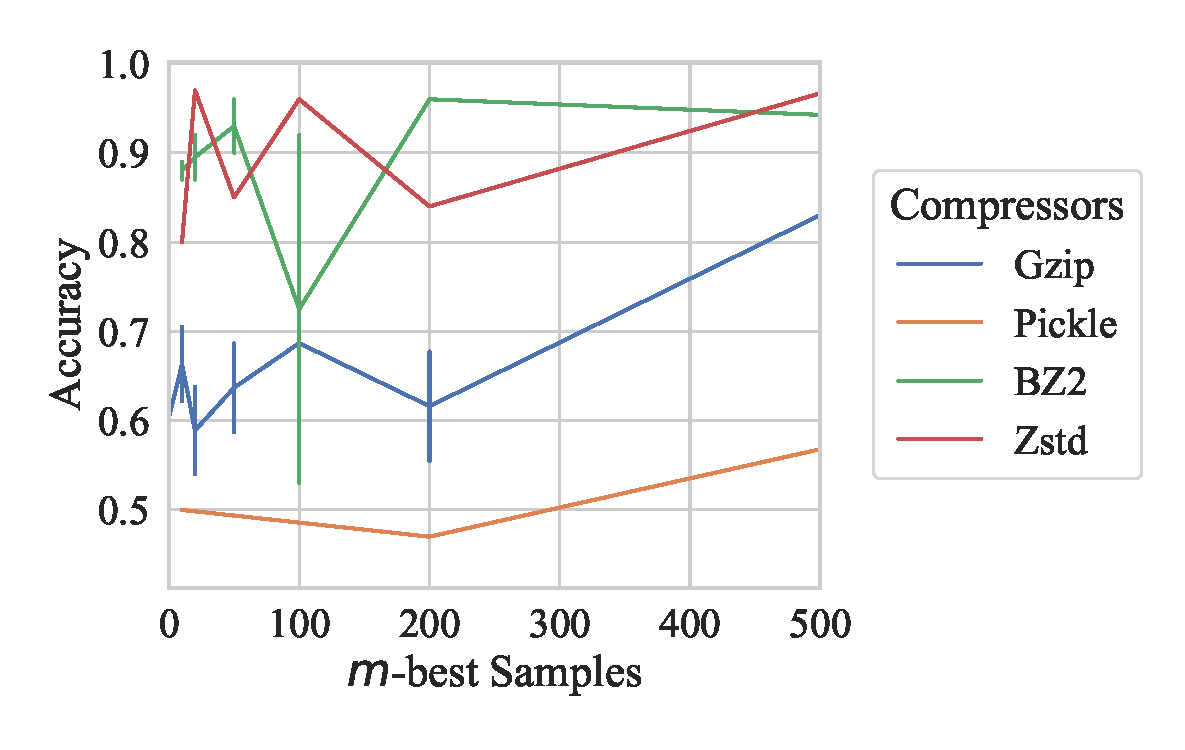
\includegraphics[width=.46\textwidth]{figs/kdd_nsl/compressor_vs_accuracy.pdf}
	% \end{subfigure}%
	% ~
	\begin{subfigure}
		\centering
		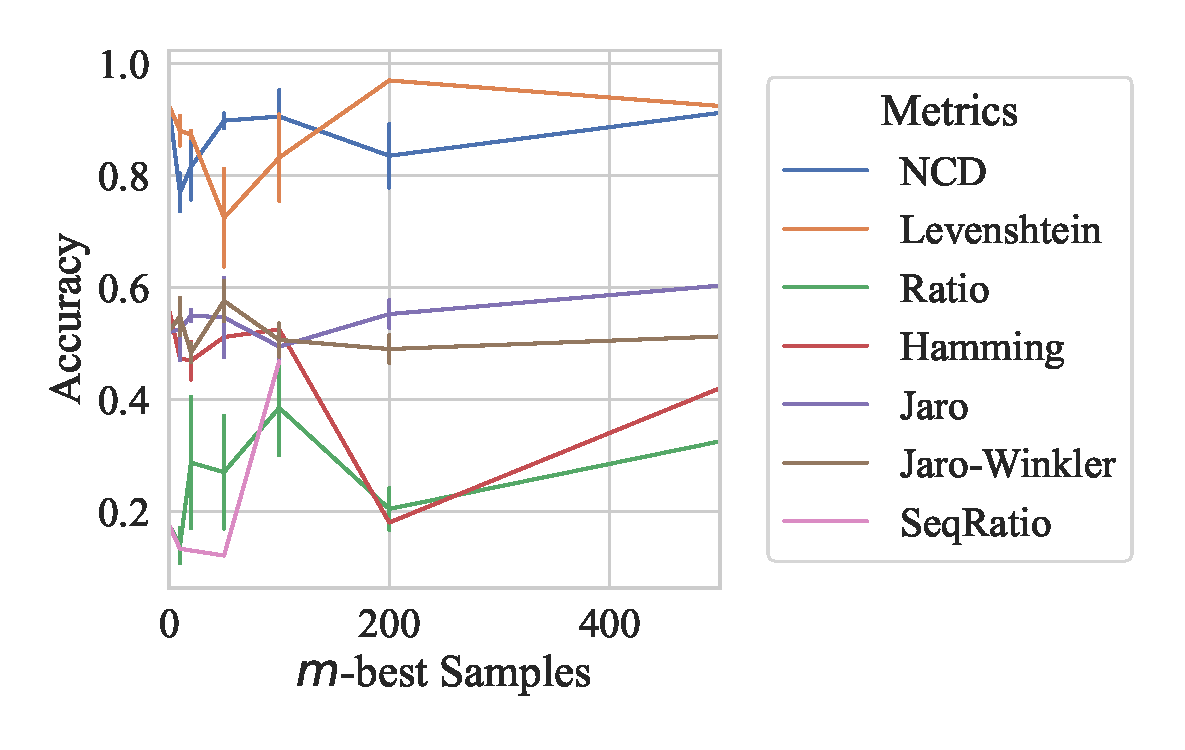
\includegraphics[width=.46\textwidth]{figs/kdd_nsl/metric_vs_accuracy.pdf}
	\end{subfigure}
	~
	\begin{subfigure}
		\centering
		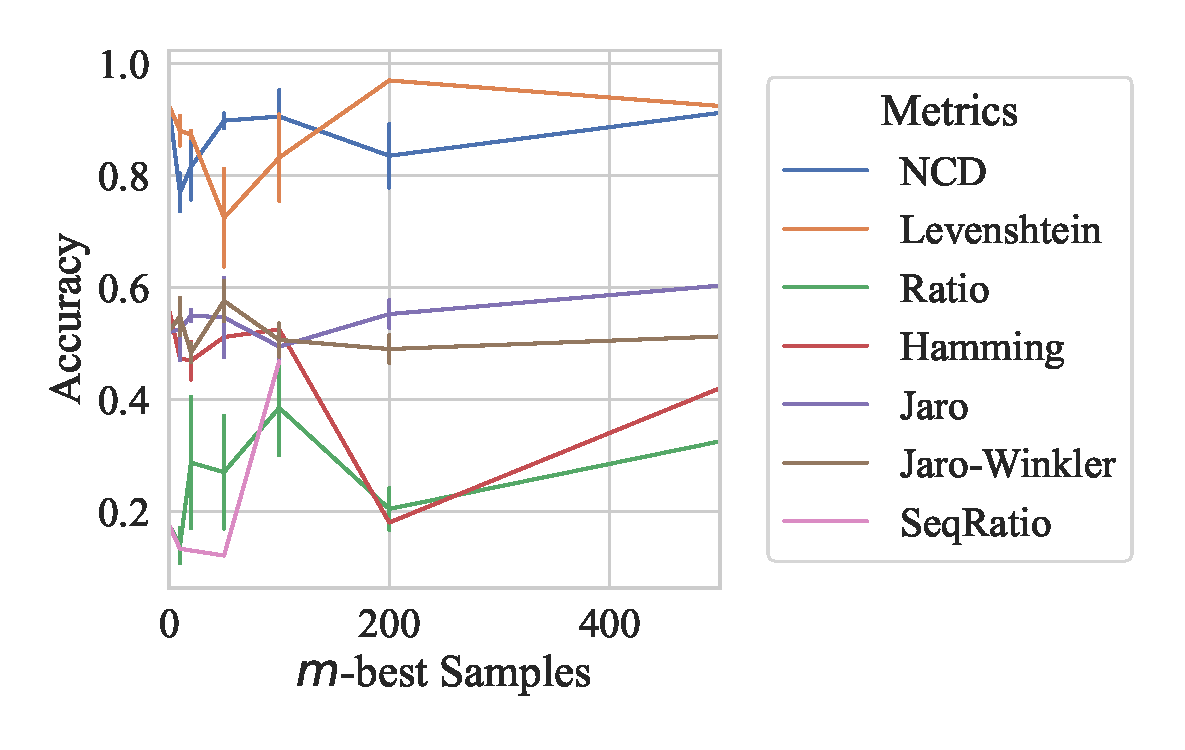
\includegraphics[width=.46\textwidth]{figs/kdd_nsl/metric_vs_accuracy.pdf}
	\end{subfigure}
	\caption{Accuracy across different different string kernel metrics (left), and sampling methods (right).}
	\label{fig:accuracy_kdd}
\end{figure*}

\subsubsection{Training Time}

Figure~\ref{fig:training_time} depicts the training time across all the tested compressors, distance metrics, and sample selection methods.

\begin{figure*}
	% \begin{subfigure}
	% 	\centering
	% 	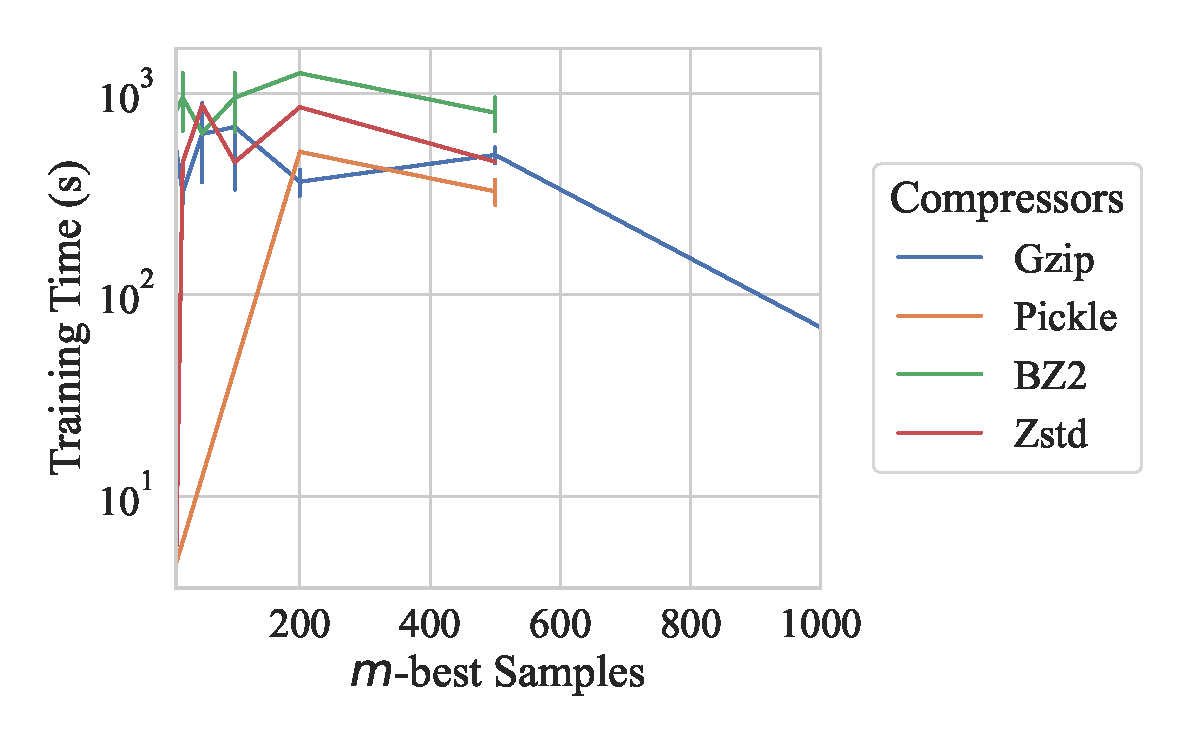
\includegraphics[width=.46\textwidth]{figs/kdd_nsl/compressor_vs_train_time.pdf}
	% \end{subfigure}%
	% ~
	\begin{subfigure}
		\centering
		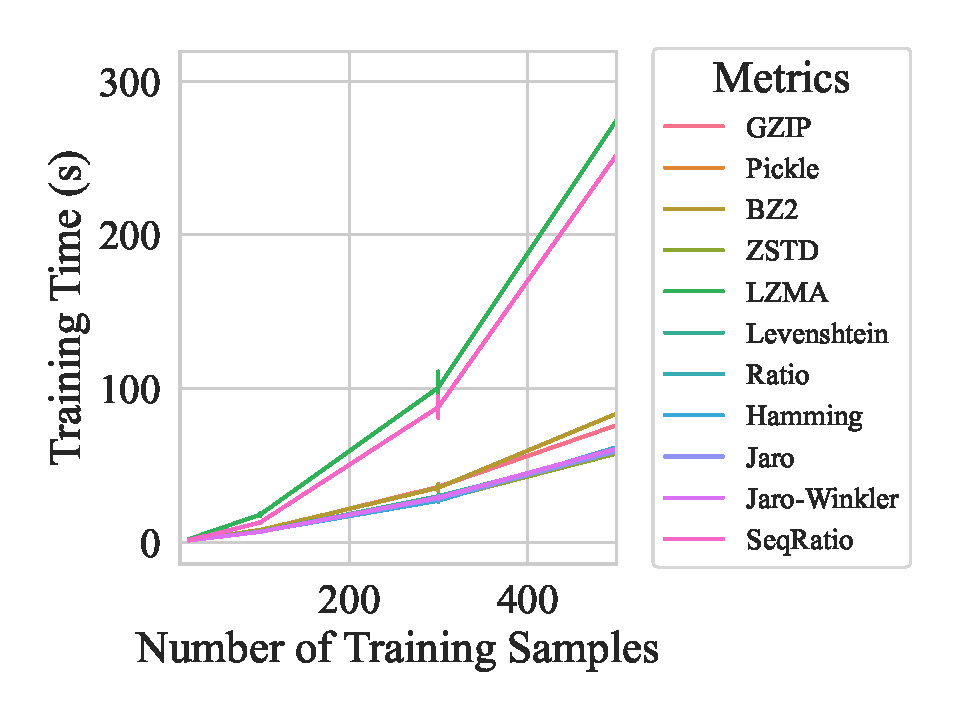
\includegraphics[width=.46\textwidth]{figs/kdd_nsl/metric_vs_train_time.pdf}
	\end{subfigure}
	~
	\begin{subfigure}
		\centering
		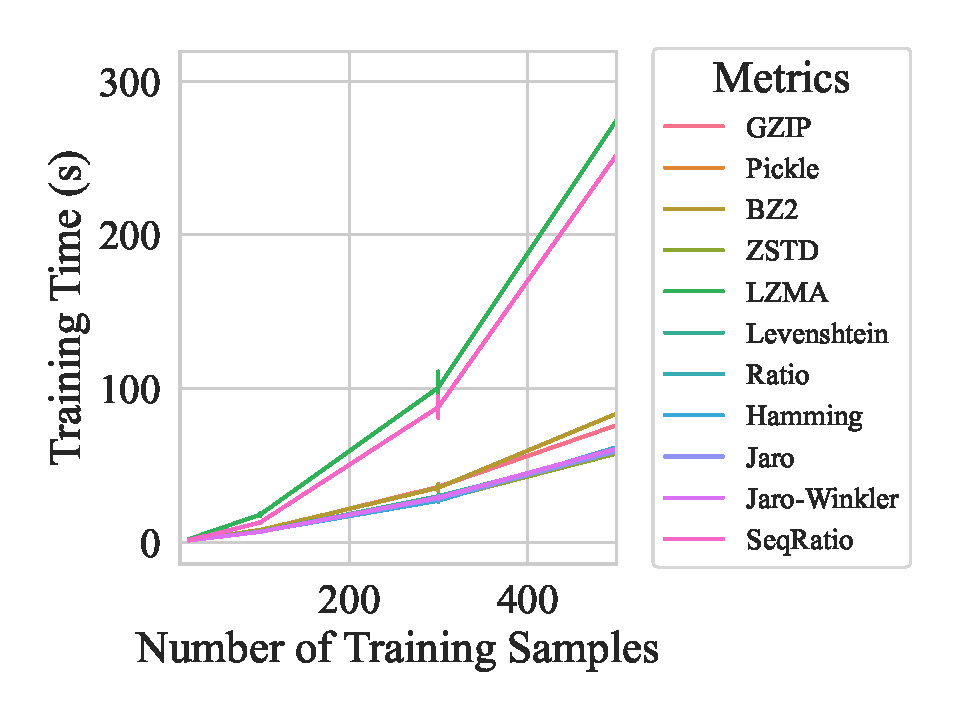
\includegraphics[width=.46\textwidth]{figs/kdd_nsl/metric_vs_train_time.pdf}
	\end{subfigure}
	\caption{Training time across different different string kernel metrics (left), and sampling methods (right).}
	\label{fig:training_time_kdd}
\end{figure*}

\subsubsection{Prediction Time}

Figure~\ref{fig:prediction_time} shows the prediction time of different compressors, metics, and sample selection methods.
\begin{figure*}
	% \begin{subfigure}
	% 	\centering
	% 	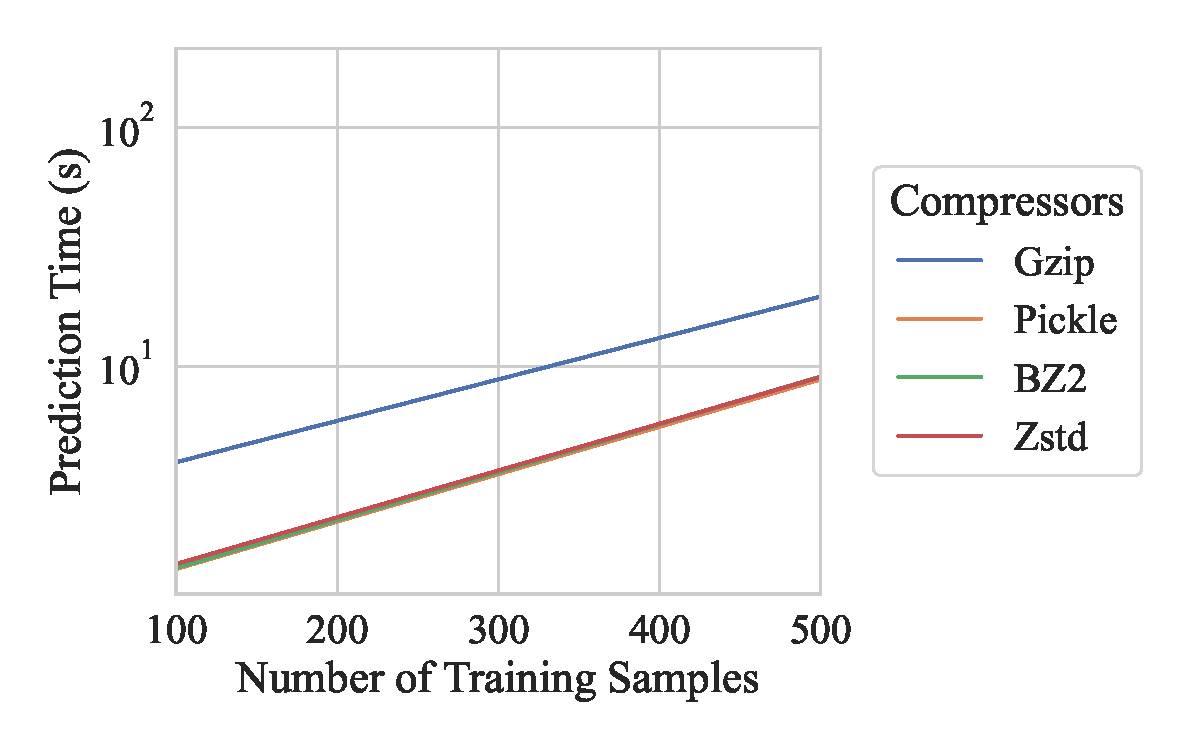
\includegraphics[width=.46\textwidth]{figs/kdd_nsl/compressor_vs_predict_time.pdf}
	% \end{subfigure}%
	% ~
	\begin{subfigure}
		\centering
		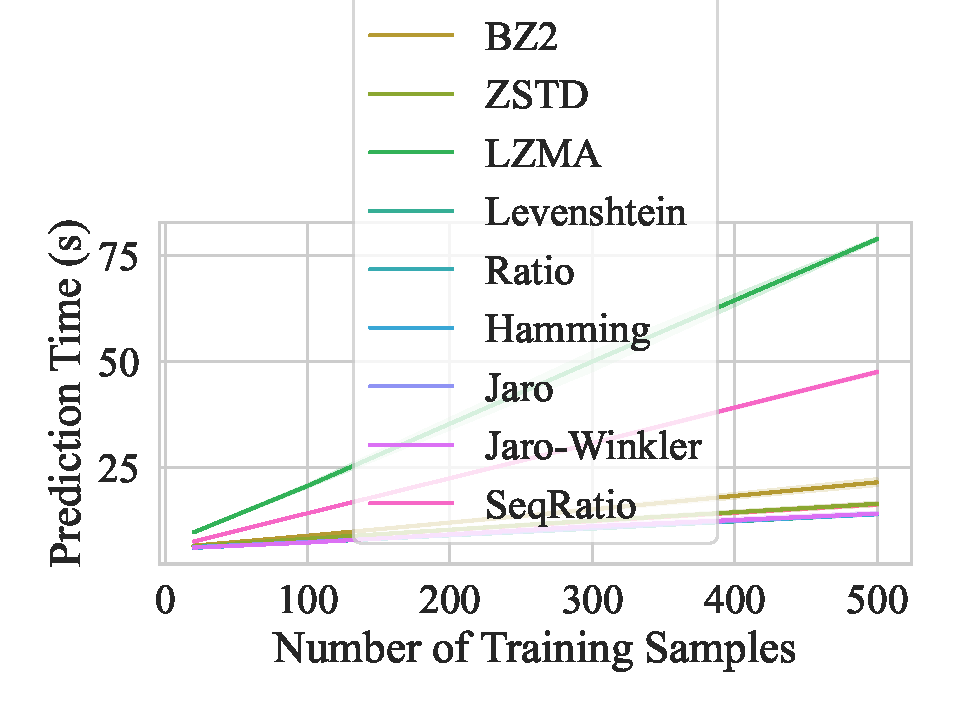
\includegraphics[width=.46\textwidth]{figs/kdd_nsl/metric_vs_predict_time.pdf}
	\end{subfigure}
	~
	\begin{subfigure}
		\centering
		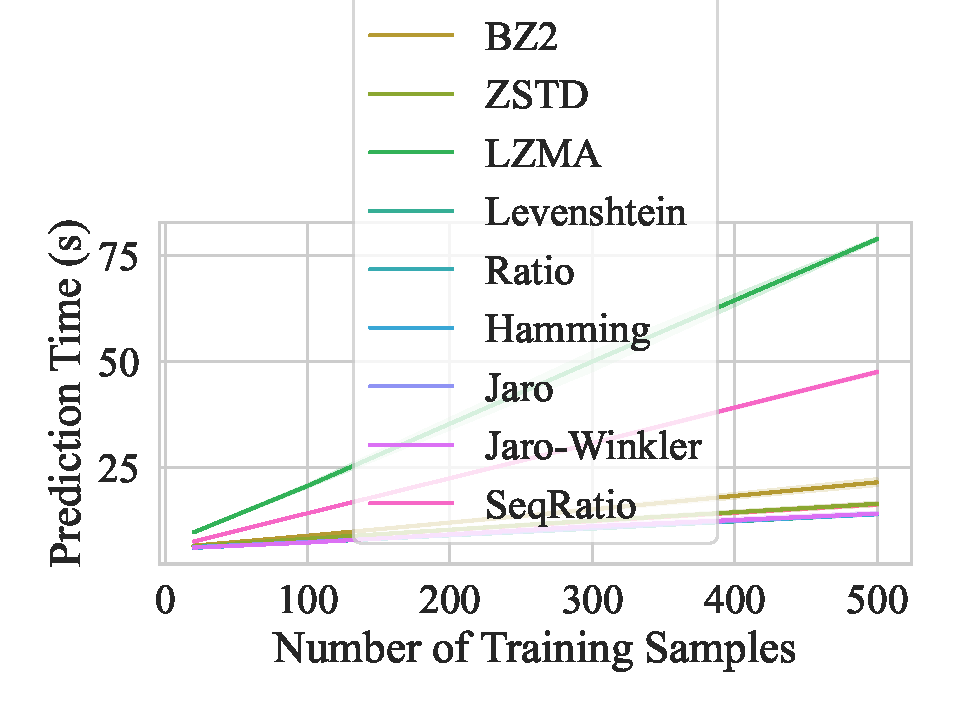
\includegraphics[width=.46\textwidth]{figs/kdd_nsl/metric_vs_predict_time.pdf}
	\end{subfigure}
	\caption{Prediction time across different different string kernel metrics (left), and sampling methods (right).}.
	\label{fig:prediction_time_kdd}
\end{figure*}

\subsubsection{Symmetry}


\begin{figure*}
    % \begin{subfigure}
    %     \centering
    %     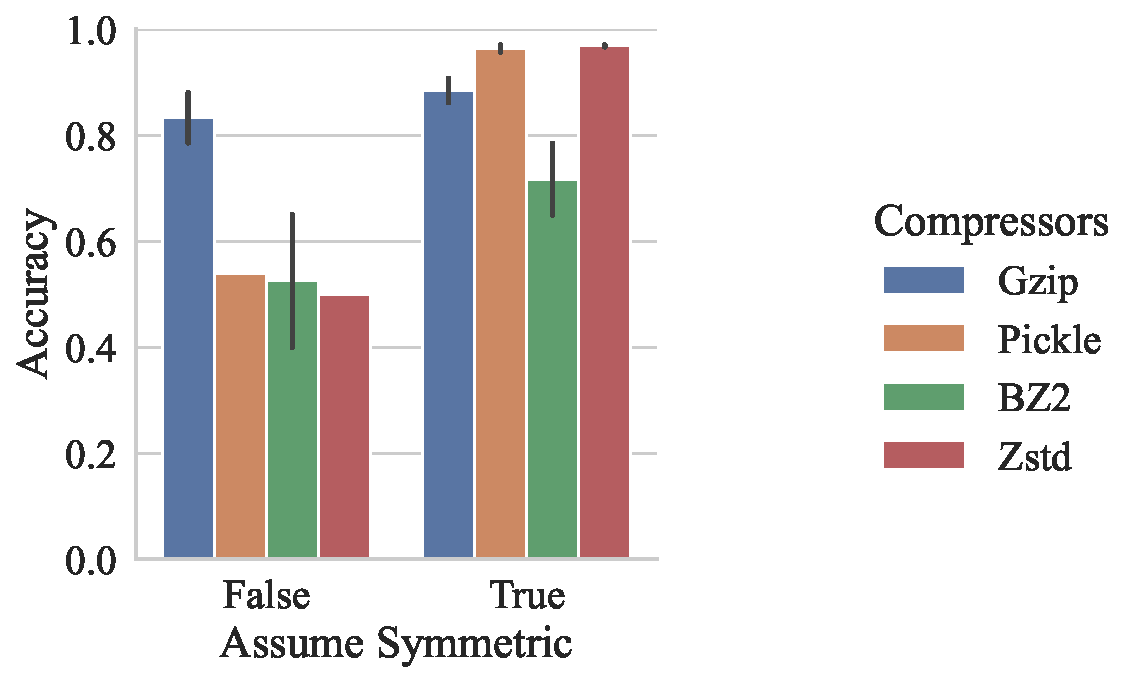
\includegraphics[width=.36\textwidth]{figs/truthseeker/symmetric_vs_compressor.pdf}
    % \end{subfigure}
    \begin{subfigure}
        \centering
        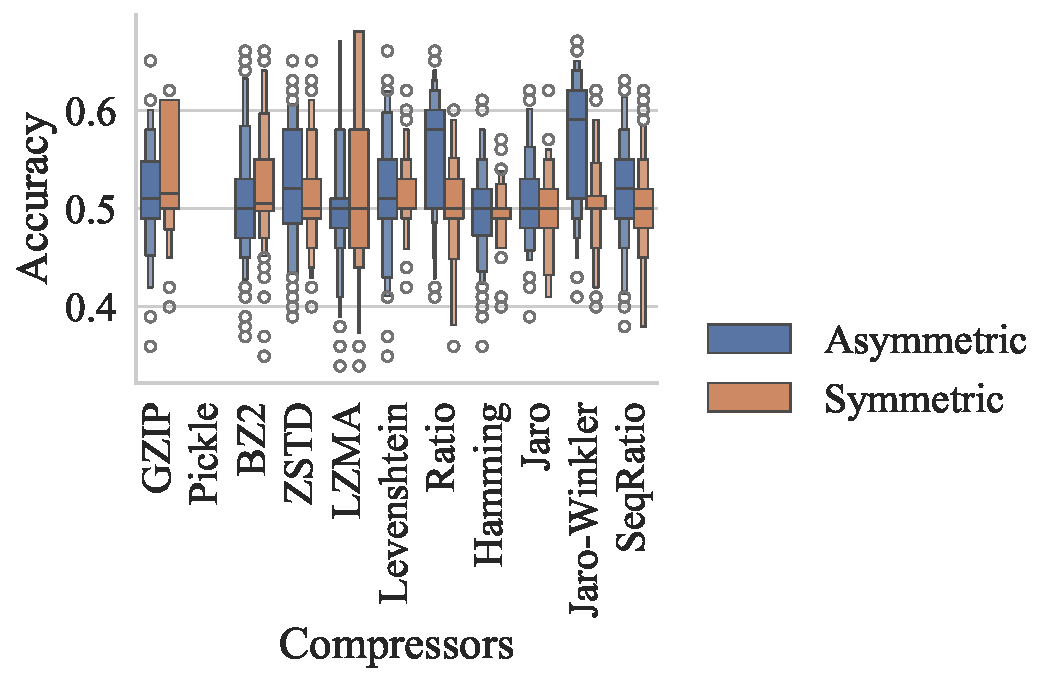
\includegraphics[width=.36\textwidth]{figs/truthseeker/symmetric_vs_metric.pdf}
    \end{subfigure}
    \begin{subfigure}
        \centering
        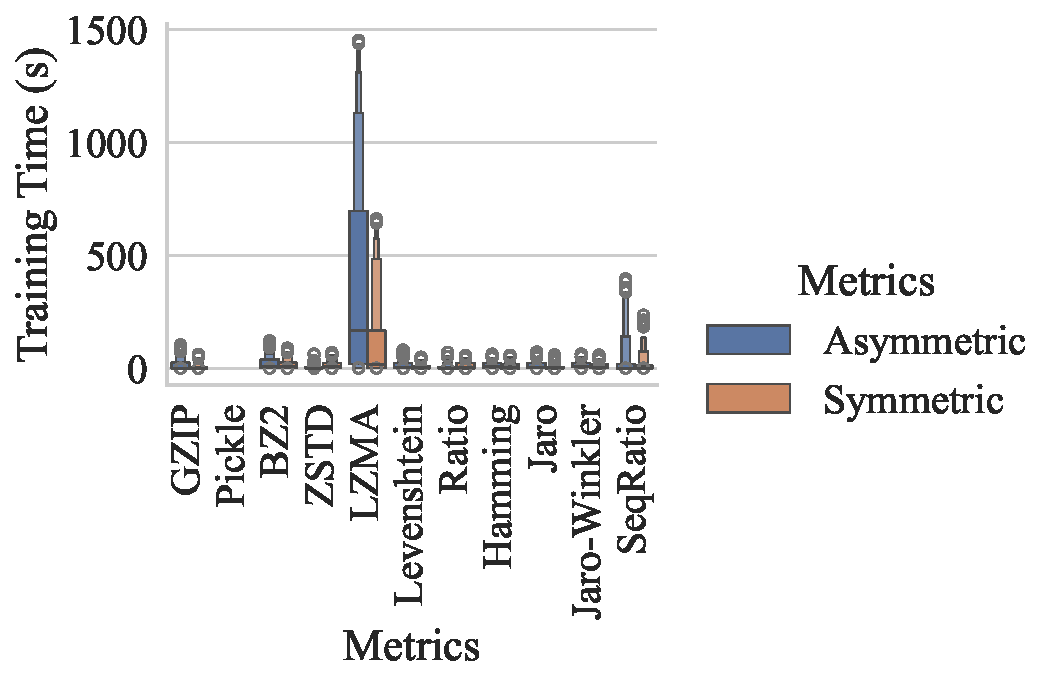
\includegraphics[width=.36\textwidth]{figs/truthseeker/symmetric_vs_metric_train_time.pdf}
    \end{subfigure}
    \caption{Accuracy across (left) and prediction time (right) across several compression methods and distance metrics with and without assuming symmetric distances.}
    \label{fig:symmetry}
\end{figure*}